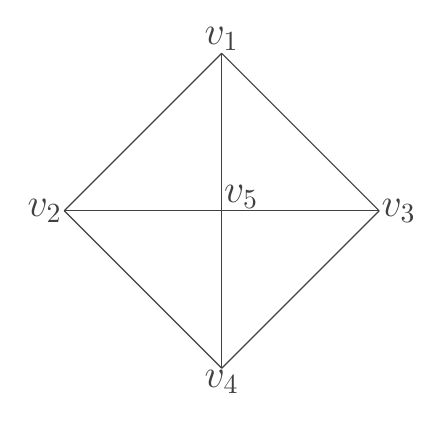
\begin{tikzpicture}[draw=darkgray, text=darkgray, align=center, node distance=2cm]
    \tikzstyle{every node}=[inner sep=0pt];

    \node (v5) [label=above right:{\Large $v_5$}] {};
    \node (v1) [label=above:{\Large $v_1$}, above of = v5] {};
    \node (v2) [label=left:{\Large $v_2$}, left of = v5] {};
    \node (v3) [label=right:{\Large $v_3$}, right of = v5] {};
    \node (v4) [label=below:{\Large $v_4$}, below of = v5] {};

    \path (v1.center)
        edge (v2.center)
        edge (v3.center);
    \path (v4.center)
        edge (v2.center)
        edge (v3.center);
    \path (v5.center)
        edge (v1.center)
        edge (v2.center)
        edge (v3.center)
        edge (v4.center);
\end{tikzpicture}
